

\documentclass{beamer}
\usetheme{metropolis}      

\usepackage[english,ukrainian,russian]{babel}
\usepackage[dvipsnames]{xcolor}
\usepackage{xcolor}
\usepackage{graphicx}




\colorlet{Mycolor1}{green!10!orange!90!}


\title{Презентація Дениска Олександра}
\date{31.05.2020}
\institute{\center"Київський політехнічний інститут імені Ігоря Сікорського" \\ група ДП-82\\студент II  курсу\\ Факультету Електроніки
}

%\author{Matthias Vogelgesang}
%\institute{"Київський політехнічний інститут імені Ігоря Сікорського"}
\begin{document}
  \maketitle
  \section
  {2) \small{Опишіть міждисциплінарний (мультифізичний) характер функціонування мікромеханічних пристроїв. Запишіть відповідні фізичні величини в рамках уявлень про електричні, гідравлічні та теплові аналогії .
}}
  
  
  
  \begin{frame}{МЕМС}
  Мікроелектромеханічні системи, МЕМС (англ. MEMS) — технології і пристрої, що поєднують в собі мікроелектронні і мікромеханічні компоненти. МЕМС-пристрої зазвичай виготовляють на кремнієвій підкладці за допомогою технології мікрообробки, аналогічно технології виготовлення однокристальних інтегральних мікросхем. Типові розміри мікромеханічних елементів лежать в діапазоні від 1 мікрометра до 100 мікрометрів, тоді як розміри кристала МЕМС мікросхеми мають розміри від 20 мікрометрів до одного міліметра.  
  \end{frame}
  
  
\begin{frame}{Застосування}
В даний час МЕМС технології вже застосовуються для виготовлення різних мікросхем. Так, МЕМС-осцилятори в деяких застосуваннях замінюють кварцові генератори. МЕМС технології застосовуються для створення різноманітних мініатюрних датчиків, таких як акселерометри, датчики кутових швидкостей, гіроскопи, магнітометричні датчики, барометричні датчики, аналізатори середовища (наприклад для оперативного аналізу крові).
  \end{frame}



\begin{frame}{Виготовлення з \textcolor{Mycolor1}{кремнію} та \textcolor{cyan}{полімеру}}
\begin{itemize}
  \item \textcolor{cyan}{МЕМС пристрої можуть бути зроблені з полімерів за допомогою таких процесів, як литтєве формування, штампування або стереолітографія; вони особливо добре підходять для застосування при виготовленні мікрофлюідних пристроїв, таких, як одноразові картриджі аналізу крові.
  \item \textcolor{Mycolor1}{ Кремній має значні переваги перед іншими матеріалами завдяки своїм фізичним властивостям. Монокристал кремнію майже ідеально підкоряється закону Гука. Це означає, що при деформації він не схильний гістерезису і, отже, енергія деформації практично не розсіюється. Основні методи отримання всіх МЕМС-пристроїв на основі кремнію: осадження шарів матеріалу, структурування цих шарів за допомогою фотолітографії і травлення для створення необхідної форми.}
 }
 \end{itemize}

  \end{frame}


\begin{frame}
  
  \section
  {12) \small{Мікромеханічні первинні перетворювачі температури на основі р-n переходу. Запишіть вольт-амперну характеристику р-n переходу та отримайте з неї залежність напруги від температури при заданому струмі. Наведіть ескіз такого первинного перетворювача. }}
\end{frame}




\begin{frame}{Перетворювачі температури на основі р-n переходу}
 У термосенсорах, що випускаються фірмою Analog Devices, які виконані за інтегральною технологією, як термочутливий сенсор використовується інтегральна мостова диференціальна схема. Кремнієві транзистори, що працюють у нижніх плечах моста, є термочутливими елементами (струм колекторного p-n переходу залежить від температури). Якщо зазначені транзистори працюють у режимі постійного відношення колекторних струмів r , то різниця напруг їхніх емітерно-базових переходів буде визначатися співвідношенням
 \large{ ${\rm\frac{\frac{kT}{q}}{Ln(r)} }}$, де k - постійна Больцмана,
q - заряд електрона. Крім того, величина r, обумовлена опорами в
ланцюгах емітерів термочутливих транзисторів, також постійна, а різниця напруг емітерно-базових переходів буде пропорційна температурі середовища T , у якій працюють транзистори.
  \end{frame}



\begin{frame}{Перетворювачі температури }
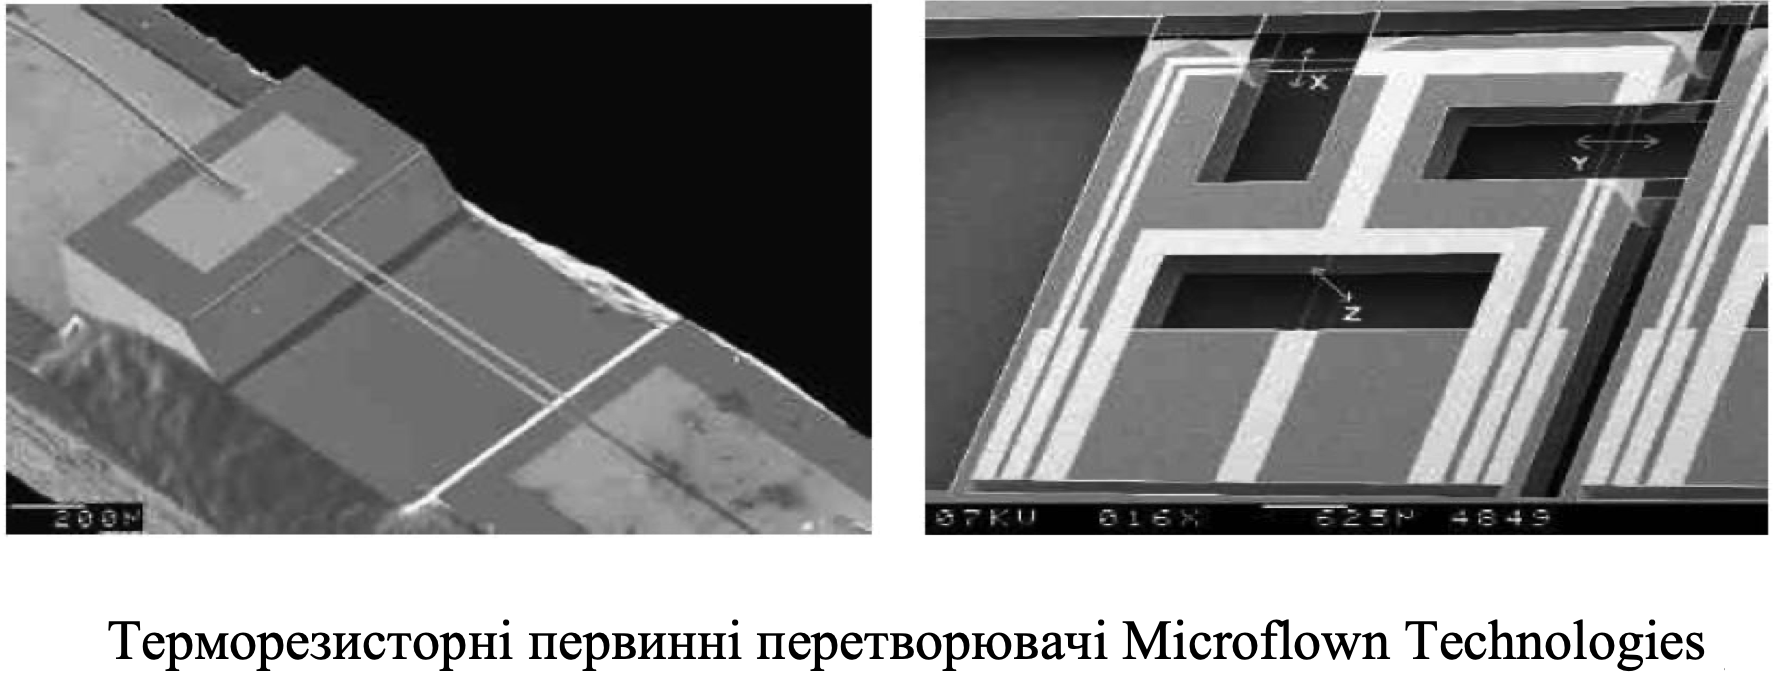
\includegraphics[scale=0.35]{s1.png}

Для виміру температури, поряд з напівпровідниковими сенсорами, що використовують температурні властивості p-n переходів застосовують термістори, що виготовлені з окисних напівпровідників. Вони забезпечують вимір у широкому діапазоні температур від –80 до 3000°С і мають високий від’ємний температурний коефіцієнт опору до –${\rm\frac{5\%}{ ^\circ C}}$. 
  \end{frame}













\begin{frame}{ВАХ для p-n переходу}
\center 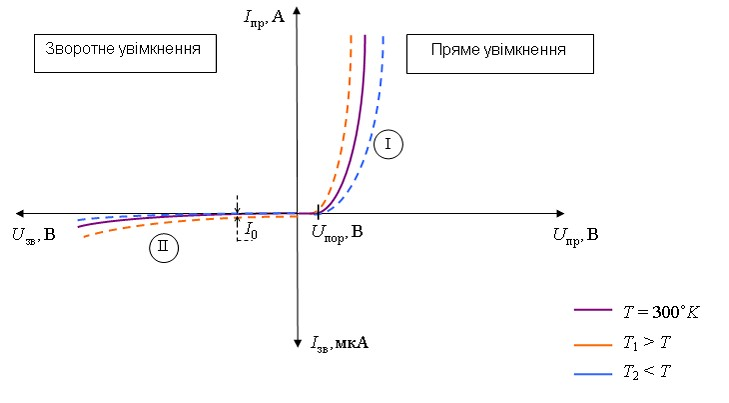
\includegraphics[scale=0.23]{svax.jpg}\\
\tiny При аналізі реальних процесів в електронно-дірковому переході потрібно використовувати вольт-амперну характеристику (рис. 1)
\center 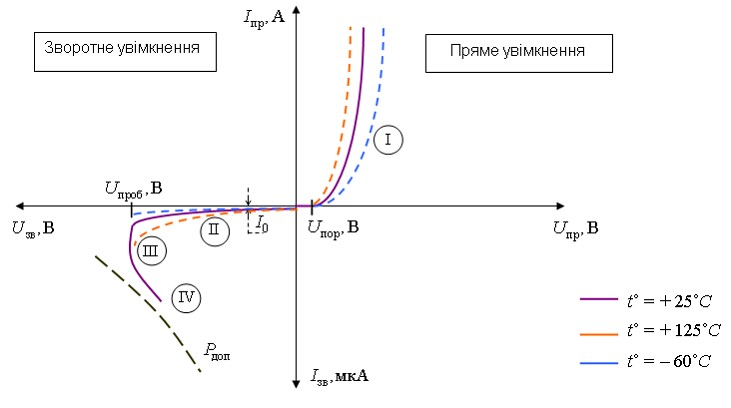
\includegraphics[scale=0.25]{s1vax.jpg}\\
\tiny (рис. 1)
\end{frame}



 
\begin{frame}{Конструкція об’ємного платинового терморезисторного перетворювача}
\center 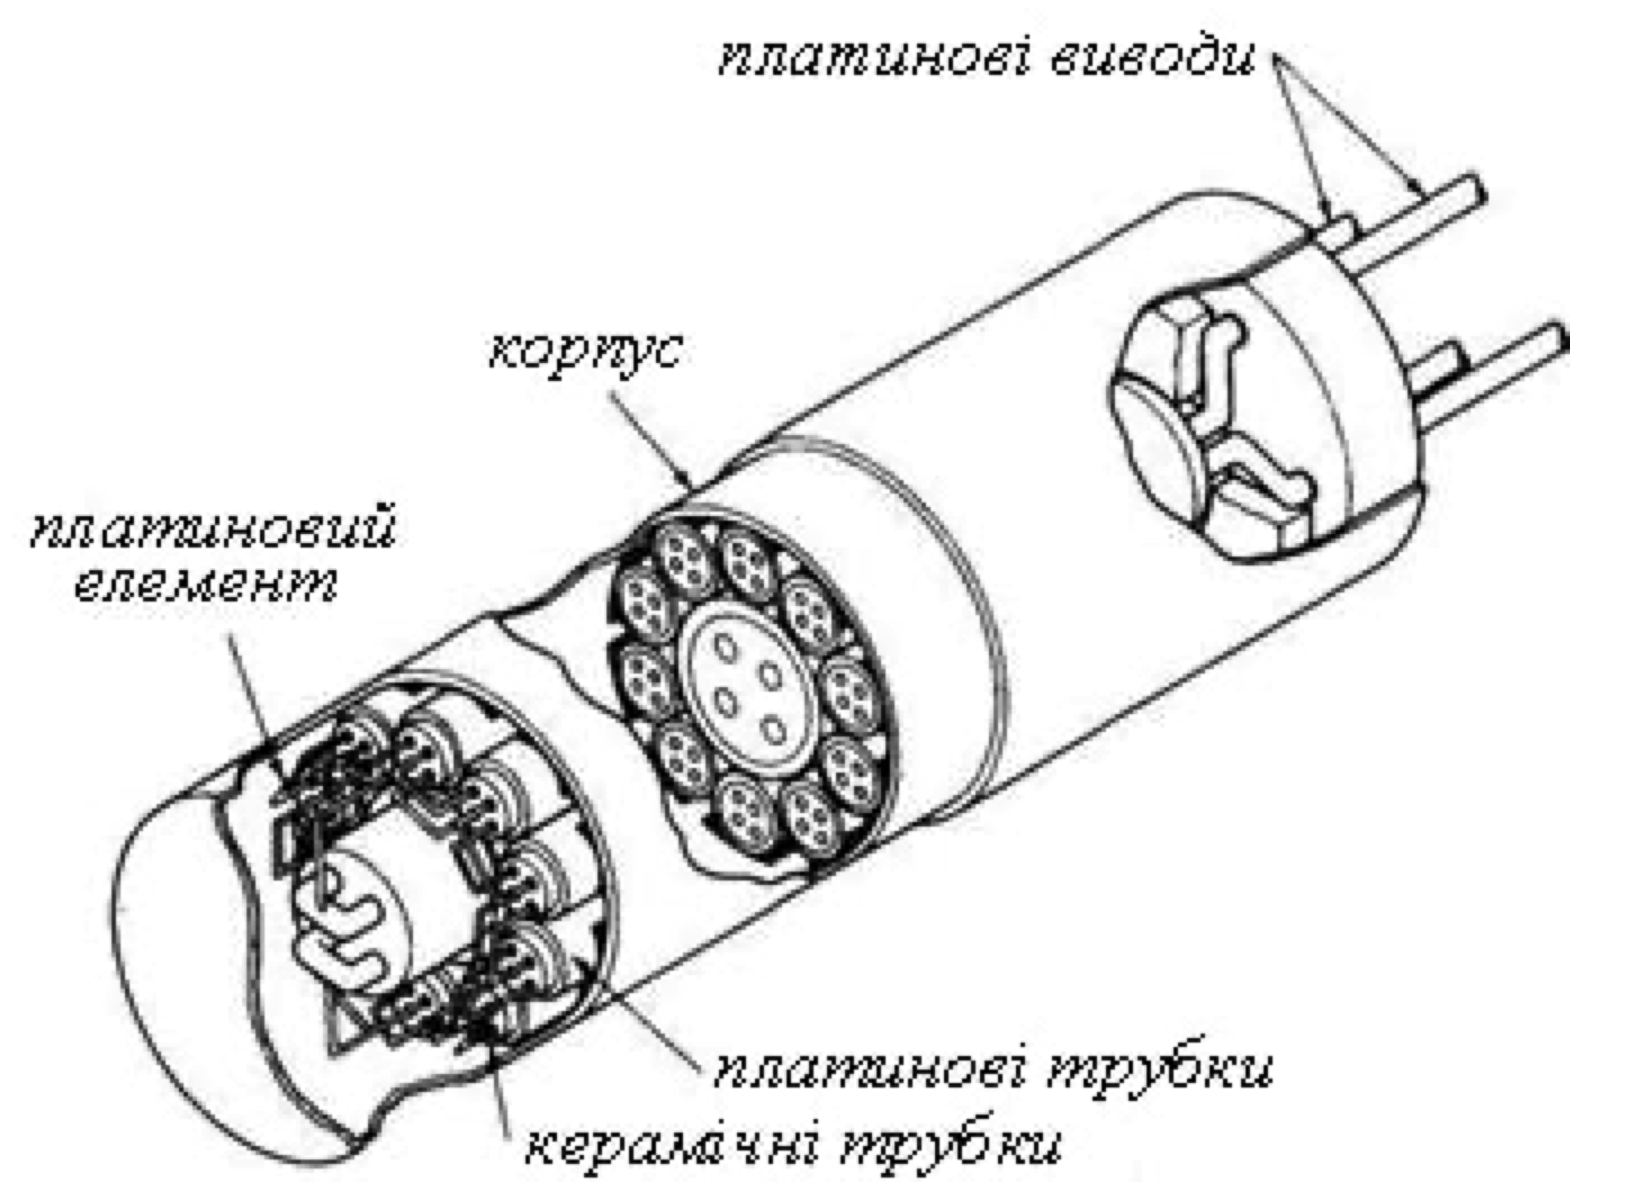
\includegraphics[scale=0.23]{trpp.png}\\
\tiny Конструкція об’ємного ТРПП (терморезисторний первинний перетворювач) традиційно складається з ТЧЕ (термочутливий елемент), захисної арматури і внутрішніх з’єднувальних провідників, комутованих за двох-, трьох- або чотирьох-провідною схемою
\end{frame}




\begin{frame}{Дротяний терморезисторний перетворювач}
\center 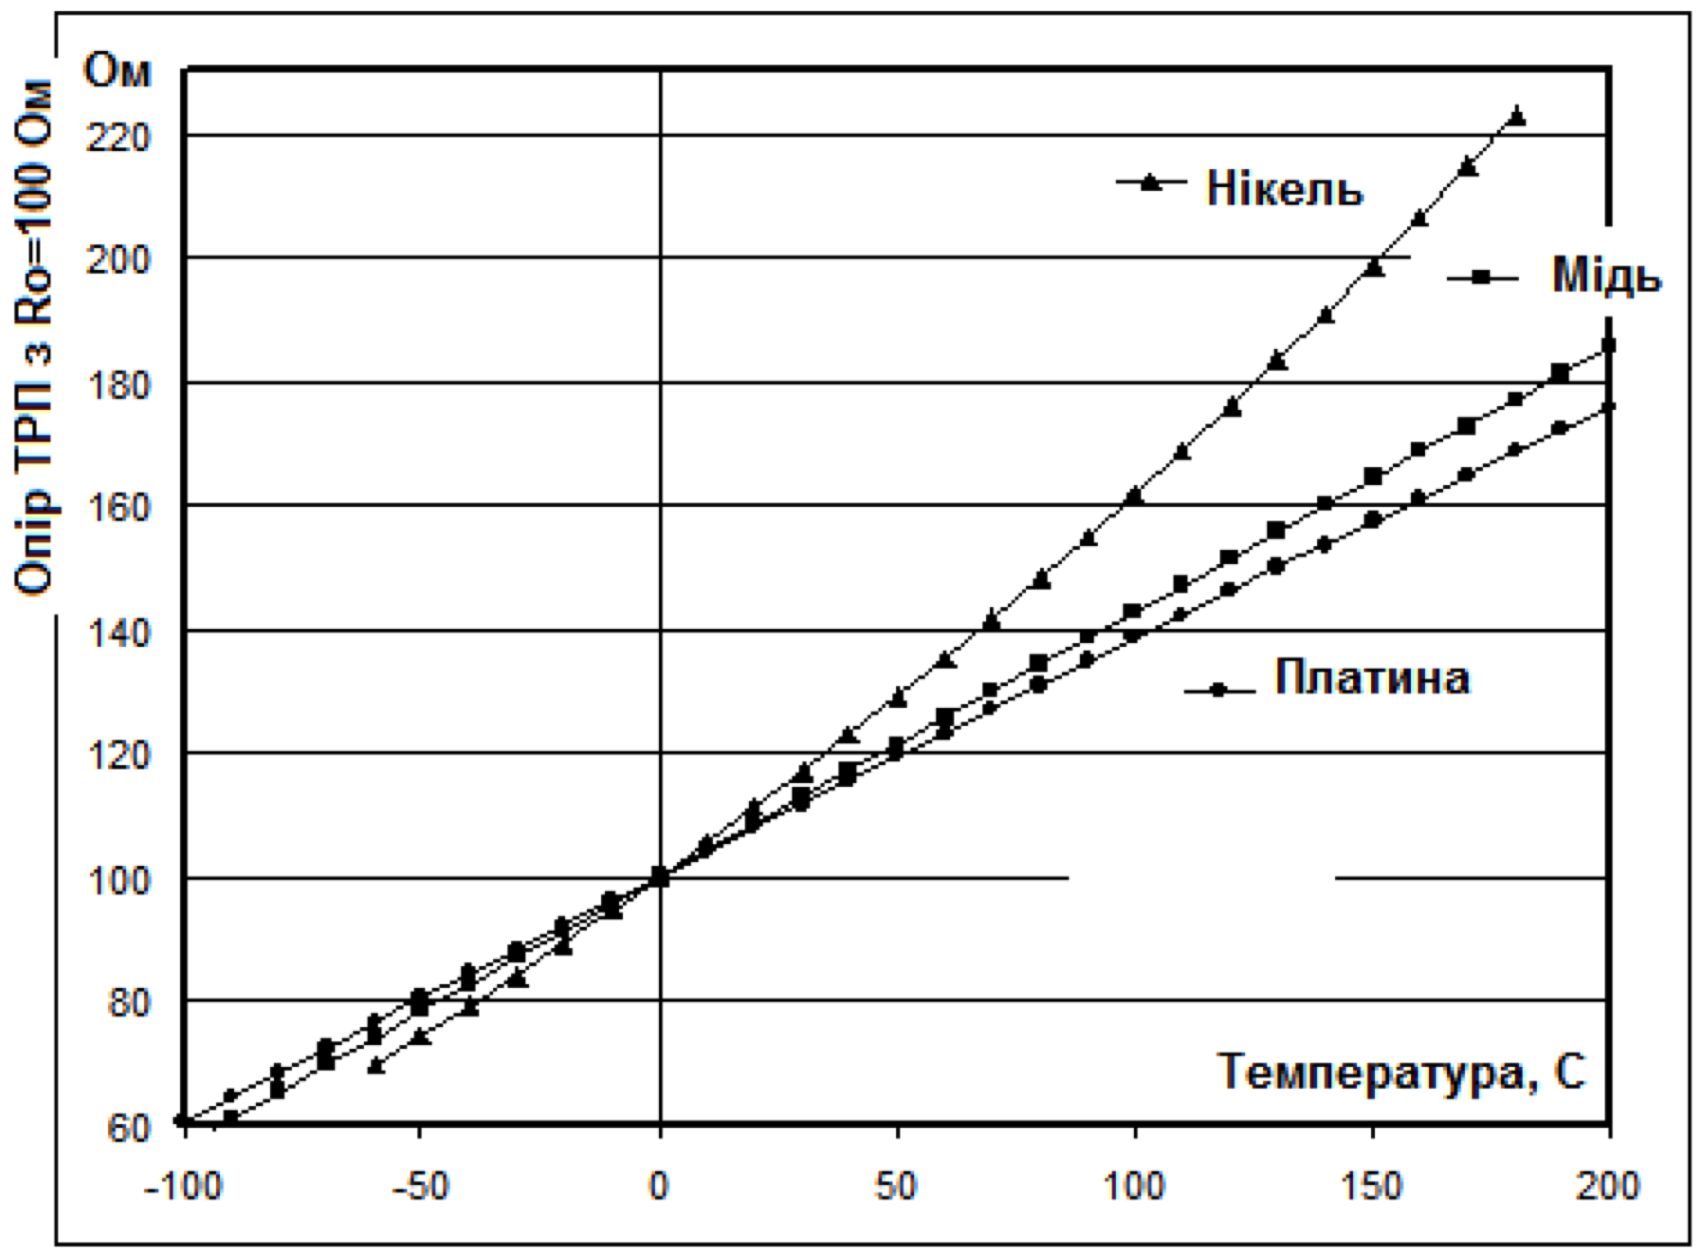
\includegraphics[scale=0.23]{trpp1.png}\\
 \smallЗалежність електричного опору дротяних терморезисторних перетворювачів від температури для платини\\ міді та нікелю при
  ${\rm R_{0}}$ = 100 Ом
 \end{frame}




\begin{frame}
  \section
  {22) \small{Наведіть приклади мостів Уітстона (резисторних вимірювальних схем), запишіть їх характеристики перетворення (залежність напруги у вимірювальній діагоналі від зміни номіналів резисторів).
 }}
\end{frame}


\begin{frame}{Вимірювальний  міст (міст Уітстона)}
\begin{center}
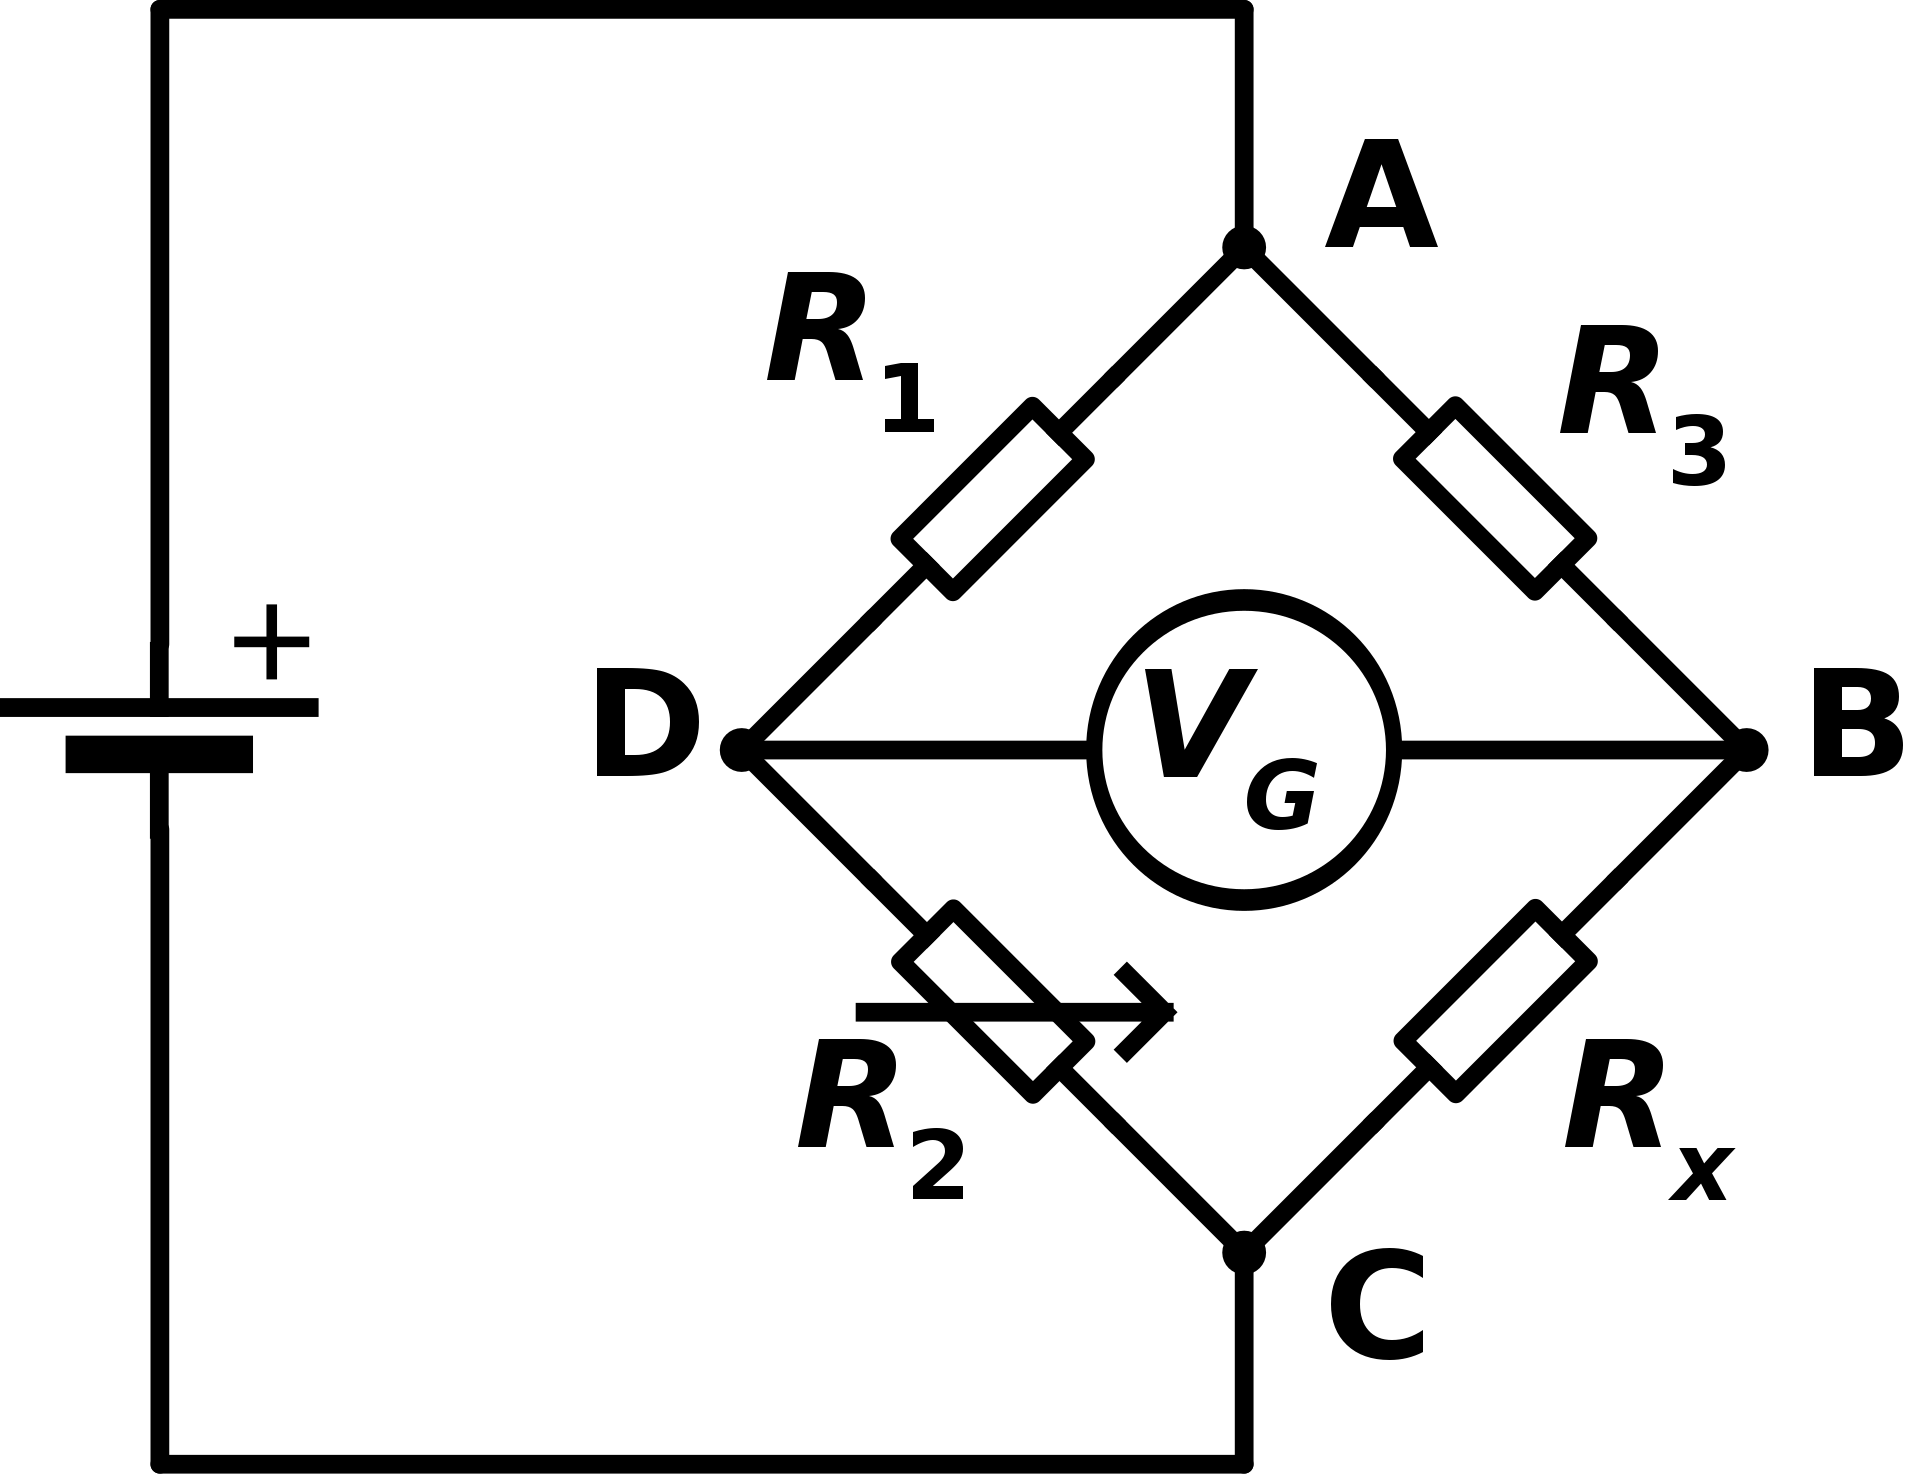
\includegraphics[scale=0.08]{most.png}\\ \textcolor{black}{Рис: схема моста Уитстона}\\
\end{center}
Міст Уитстона по суті універсальний, і застосується не лише для вимірювань опорів резисторів, але і для знаходження найрізноманітніших неелектричних параметрів, досить лише щоб сам датчик неелектричної величини був резистивним.
  \end{frame}




\begin{frame}{Застосування моста Уітстона}
\begin{center}
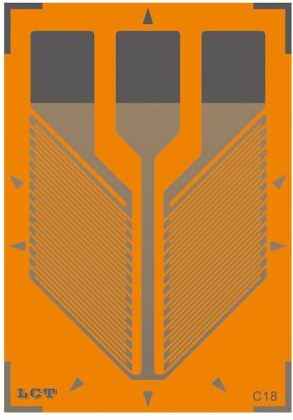
\includegraphics[scale=0.3]{dav.jpg}\\ \textcolor{blue}{Рис: датчики механічної напруги}\\
\end{center}
\small
Сучасні вимірювальні прилади на базі моста Уитстона зазвичай знімають показання з моста через аналого-цифровий перетворювач, підключений до цифрового обчислювальному пристрою, такого як мікроконтролер з вшитой програмою, яка здійснює линеаризацию (заміна нелінійних даних наближеними лінійними), масштабування і перетворення отриманих даних в чисельне значення вимірюваної неелектричної величини у відповідних одиницях виміру, а також корекцію похибок і висновок в читається цифровому вигляді.
\end{frame}
  
  
  
  
  \begin{frame}{Застосування моста Уітстона}
%\begin{center}
\center Витяг з Вікіпедії
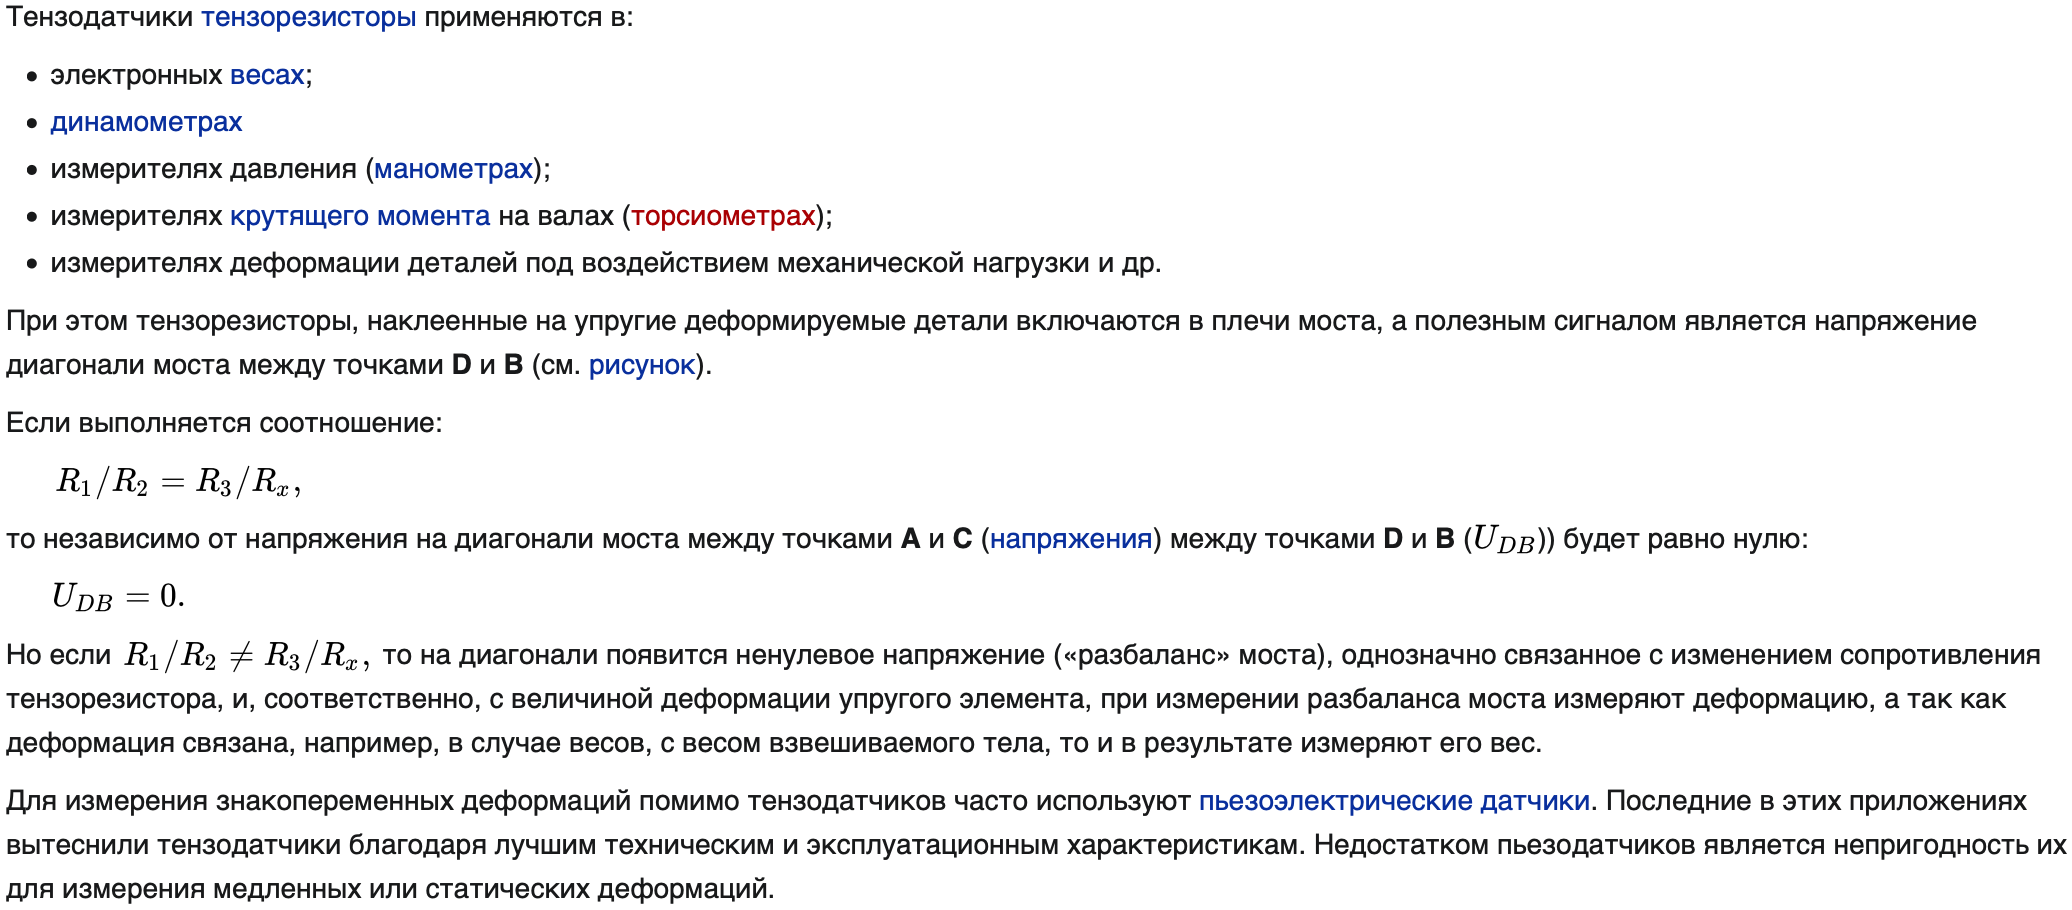
\includegraphics[width=11.5cm, heigh=12cm]{viki.png}\\ 
\hfill
%\end{center}
\small

\end{frame}
  
  
  
  
  
  
  
  
  
  \begin{frame}
  \section
  {30) \small{Назвіть області, на Ваш погляд, найбільш ефективного застосування сучасних мікроелектромеханічних систем (МЕМС) або приклади, на Ваш погляд, найбільш вдалих і перспективних комерційно доступних МЕМС у масовому виробництві. 
 }}
\end{frame}
  
  
  
  
  
  
  \begin{frame}{МЕМС датчик тиску}
 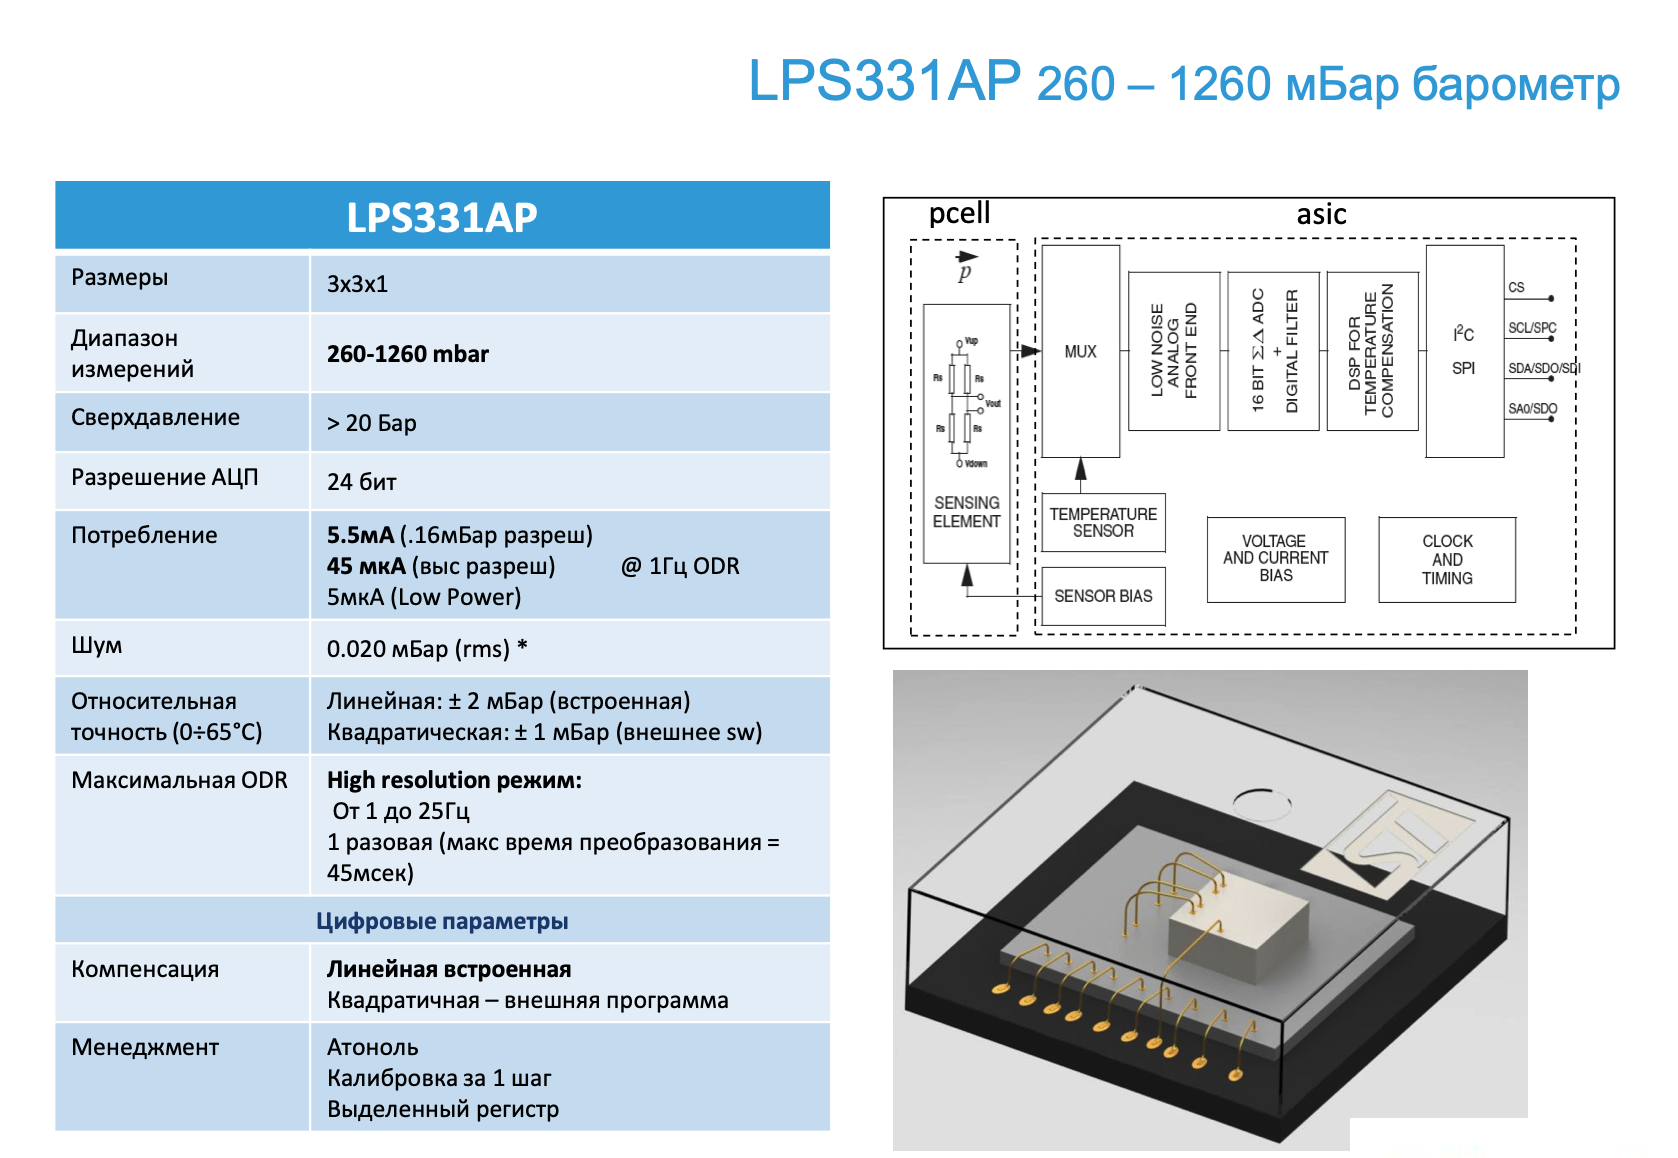
\includegraphics[width=11.5cm]{davl.png}\\ 

  {\small{ }}
\end{frame}

  
   \begin{frame}{МЕМС датчик тиску}
 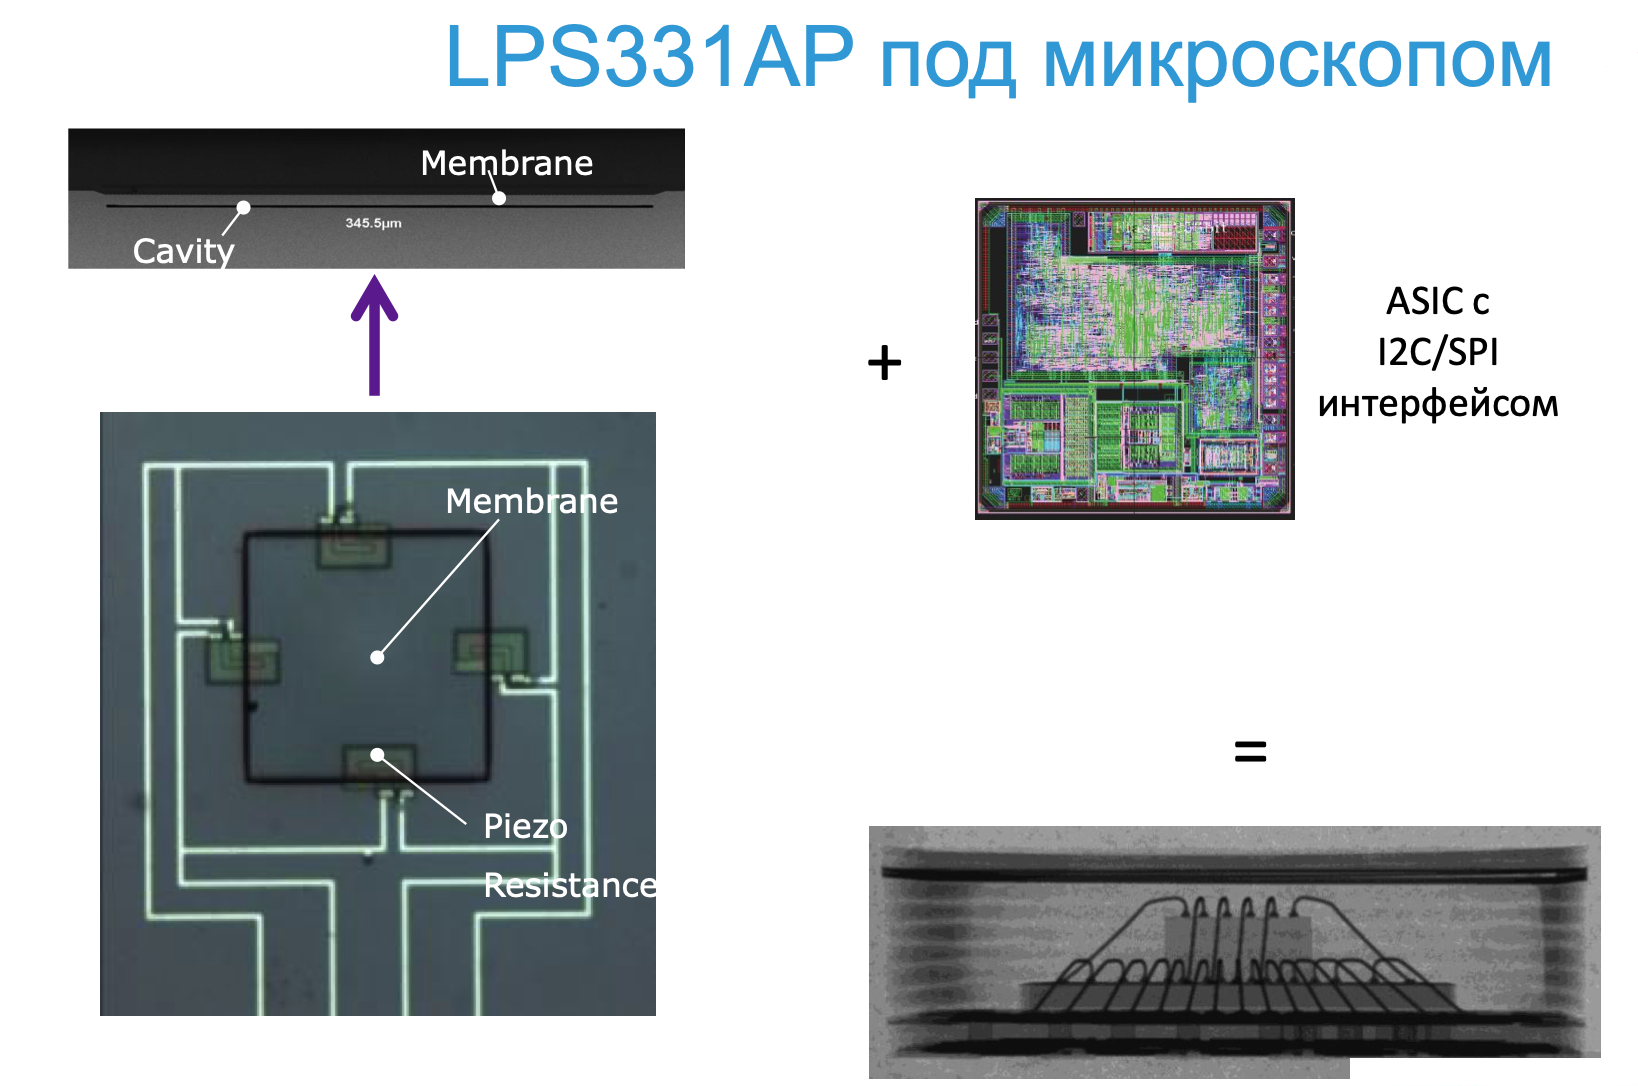
\includegraphics[width=11.5cm]{davl1.png}\\ 

  {\small{ }}
\end{frame}

  
   \begin{frame}{Приклад: сенсор оснований на роботі цього датчика}
 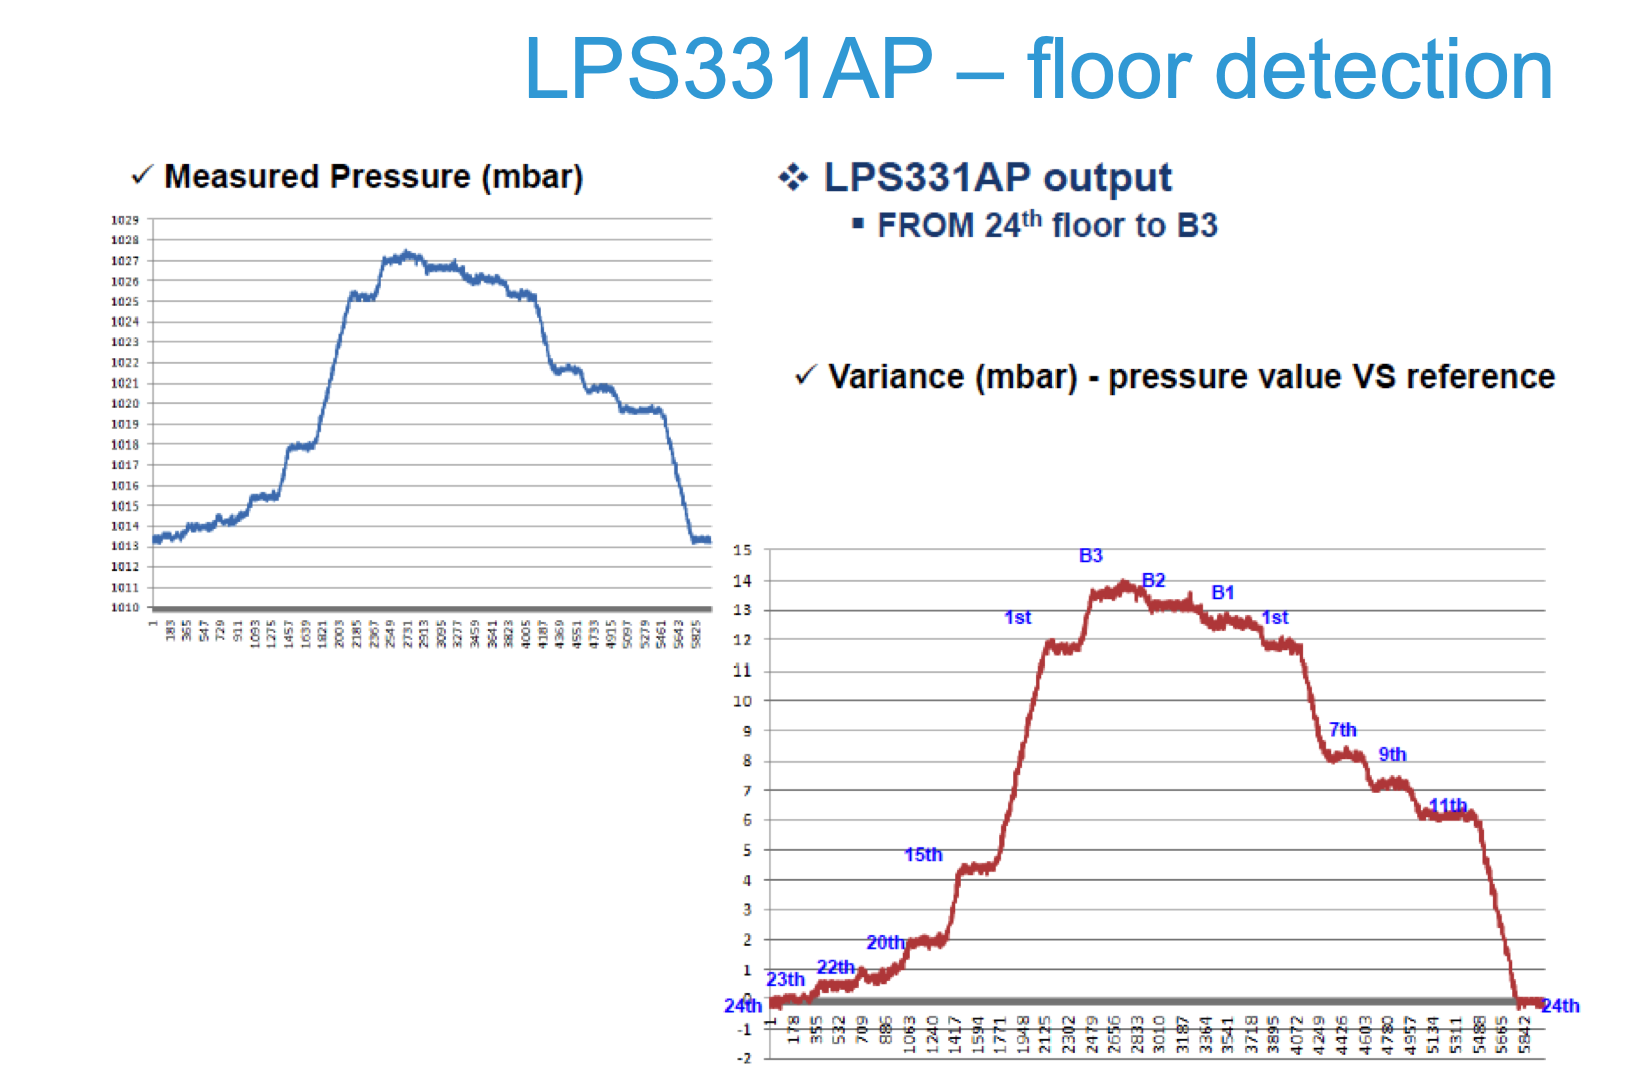
\includegraphics[width=10cm]{davl3.png}\\ 

  {\small{На графіку зображено спрацьовування  сенсора на  вагу яку на нього прикладають
(сенсор встановлений під підлогу)  }}
\end{frame}


  
  
  
  
  
  
  
\end{document}
